\subsection{Speed Estimation and Counting}
\label{subsection:count_measure}
From the bounding box subprocess the location for a foreground object for any given frame is known, therefore it is possible to measure when an object travels from one part of the image to another and how long it takes for this to occur. Vehicle counting and speed measurement is dependent on a object's position history for it is with this information that the direction and speed of movement is determined. Elements of Adrian Rosebrock's tutorial on speed estimation and tracking of vehicles were drawn on heavily for this implementation \cite{adrian_rosebrock_vehicle_tracking}. Both speed and vehicle volume measurements are stored in a database every 30 seconds. This time resolution was selected as it makes live traffic routing an effective possibility. 

\subsubsection{Counting}

Depending on the direction of travel relative to the image, that is, up or down vs side to side, a line is placed on the image which when passed by a tracked object triggers a vehicle count to increment. The direction of travel of the object is determined by averaging the history of it's centroid position where the y-values or x-values are average dependent on the direction of travel. This system assumes that vehicle will travel only vertically or horizontally relative to the edges of the camera frame.  

\begin{figure}[H]
	\centering
	\begin{subfigure}[b]{0.42\textwidth}
            \centering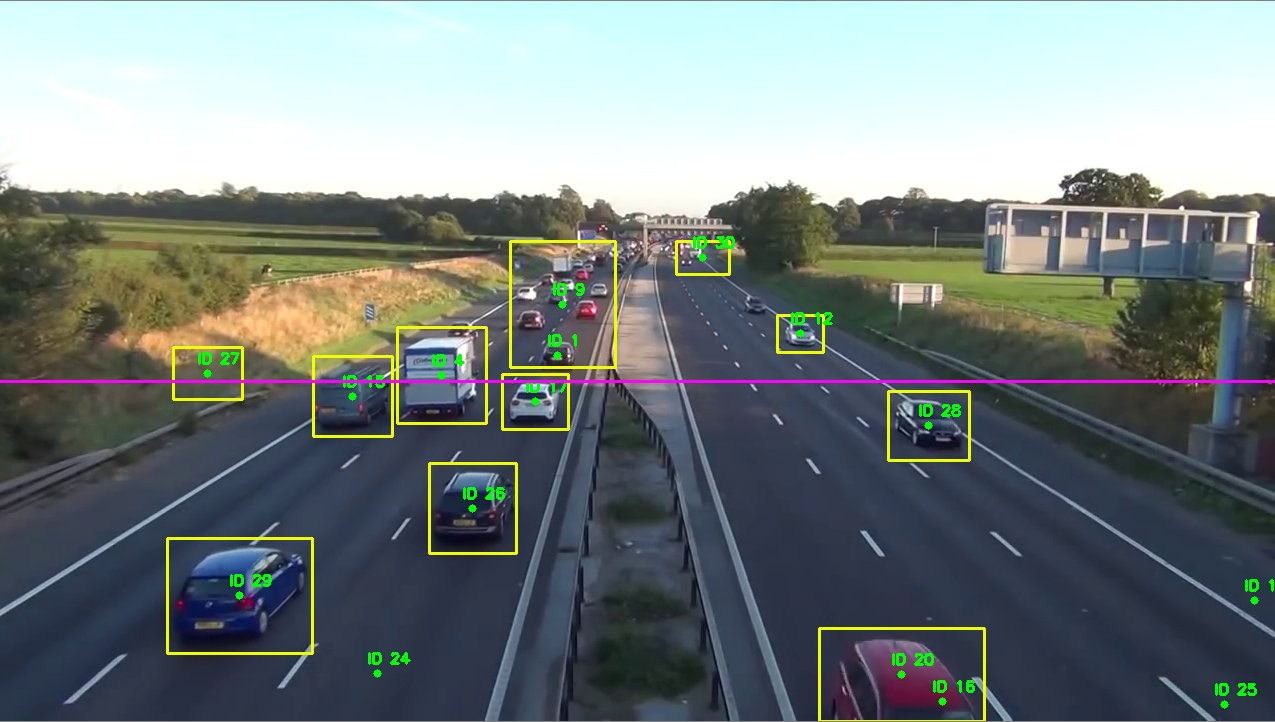
\includegraphics[width = \textwidth]{design/detection/counting/original_count}|
            \captionsetup{format = hang}  
      		\caption{Count threshold lines, bounding boxes and centroids on original frame.}
    	\end{subfigure}
    	\begin{subfigure}[b]{0.42\textwidth}
      		\centering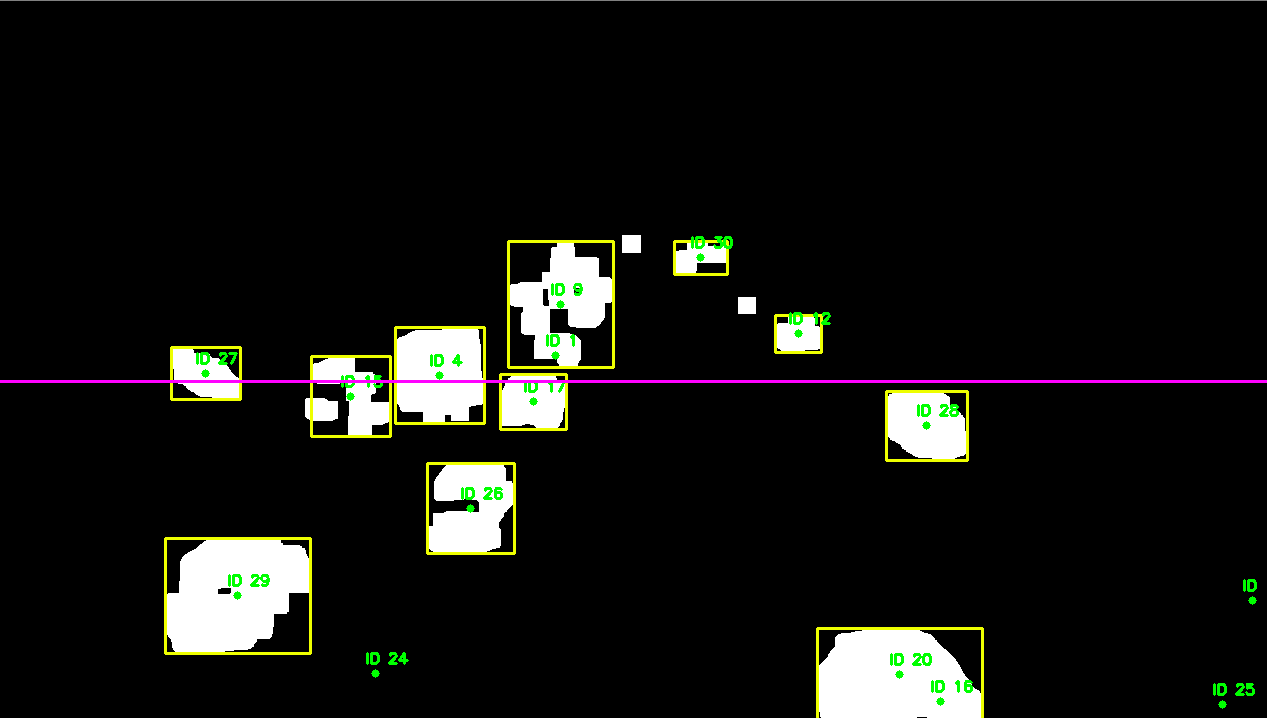
\includegraphics[width = \textwidth]{design/detection/counting/mask_count}
            \captionsetup{format = hang}    
            \caption{Count threshold lines, bounding boxes and centroids on foreground mask.}
        \end{subfigure}
        \captionsetup{format = hang}
    	\caption{Vehicle count threshold lines visualized on traffic setting and foreground mask.}
    	\label{fig:count_lines}
\end{figure}

\subsubsection{Speed Estimation}

Using the history of a centroid's location the distance the its associated object has travelled can be determined. By taking time stamps each recording it can be estimate how long it took the object to travelling from point A to B across the image and convert those distance values from pixels into some distance unit like meters an approximate speed measurement can be taken. In Figure \ref{fig:speed} the highlighted regions visualise the region between which a vehicle's speed is measure. The calibration of these regions determines the accuracy of the speed readings. For a camera perspective looking in the direction of travel as in Figure \ref{fig:original_frame} and not perpendicular to it, the accuracy will be siginificantly reduced. This is because the size of the vehicle in the frame reduces the further away it is therefore it is \emph{perceived} to travel across less pixels per time unit and conversely when it's closer it's perceived to travel faster. In a situtation where vehicles are travelling perpendicular to the camera's perspective their size remains constant and hence perceived pixels per time unit doesn't change as they move. In the former situation where a vehicle is moving towards or away from the camera it is best to select a specific region in which to measure speed between two points, where the scale of the vehicles doesn't change too much and hence limits the effect on the speed measurement. 

This type of speed measuring is referred to as \emph{Visual Average Speed Computer and Recorder} as it relies on visual inputs to determine a vehicles speed, it is less accurate than other methods like radar but is sufficient for the purpose of measuring approximate traffic speed to gauge traffic flow in conjucntion with vehicle volumes.

\begin{figure}[H]
	\centering
	\centering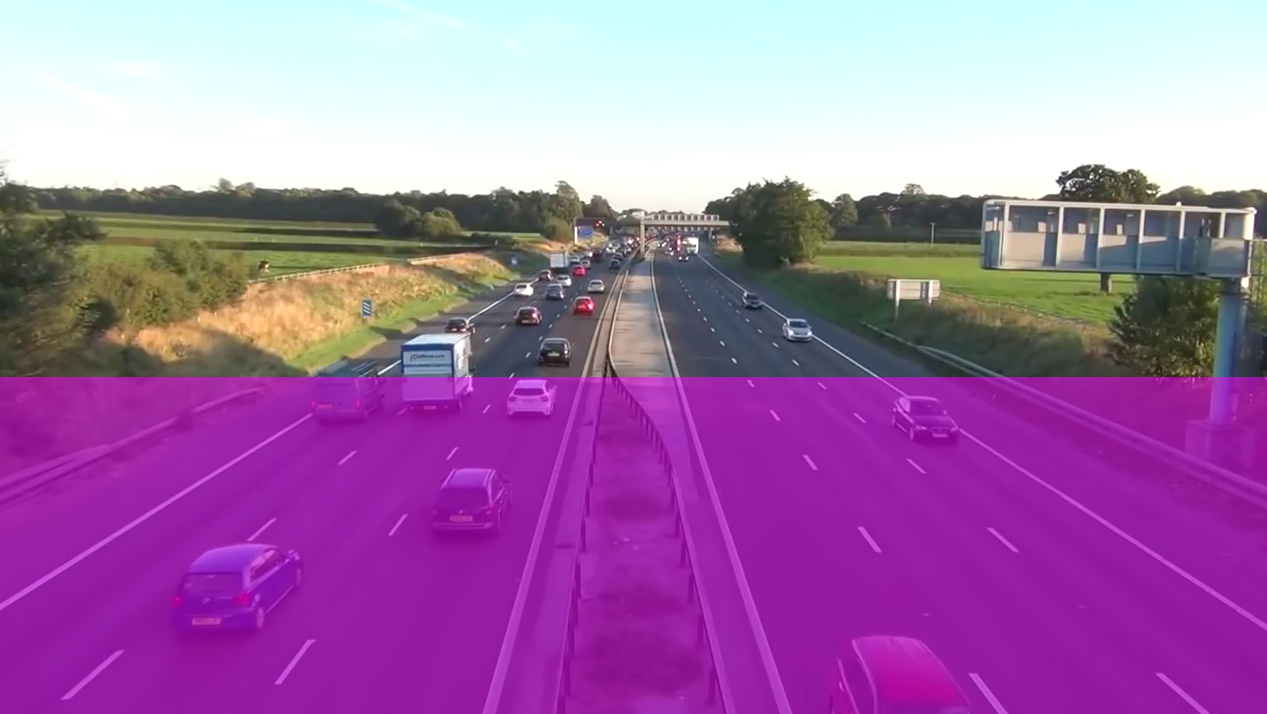
\includegraphics[width = 0.8\textwidth]{design/detection/counting/original_speed}
	\caption{Visualization of speed measurement region.}
	\label{fig:speed}
  \end{figure} 


  